\documentclass[11pt, a4paper, oneside]{mwart}

\def \MYHEADER {Projekt Bazy Danych}
\def \MYTITLE {Analizator danych pogodowych}
\def \MYPDFTITLE {term_1}
\def \MYPDFDATE {\today}
\def \MYAUTHOR {\emph{Autorzy:}\\Aleksandra~\textsc{Grzelak}\\Dorian~\textsc{Janiak}\\Marcin~\textsc{Ochman}}
\def \MYPDFAUTHOR {air}
\def \MYLECTURER {\emph{Prowadzący:} \\dr~in\.z.~G.~\textsc{Myzk}}
\def \MYLSTSETLANGUAGE {matlab}
\def \MYLSTSETFRAME {lines}
\def \MYLSTSETKEYWORDS {} 

%konfiguracja bez treści, aby podłączać do innych plików

%\usepackage[OT4,plmath,MeX]{polski}
\usepackage[utf8]{inputenc}
\usepackage[polish]{babel}
\usepackage{polski}

\usepackage{indentfirst} % polski zwyczaj dla wciec akapitowych
\usepackage{graphicx}
%\graphicspath{{../}}
\usepackage[decimalsymbol=comma]{siunitx}
\usepackage{url}
\usepackage{pdflscape} 
\usepackage{subfigure}

\usepackage{wrapfig}
\usepackage[top=3cm, bottom=3cm, left=4cm, right=4cm]{geometry}

%\oddsidemargin 0.5cm
%\evensidemargin -0.5cm

\usepackage{listings}
\renewcommand{\labelitemi}{$\circ$}


\usepackage{caption}
\usepackage{color}
\usepackage{rotating}
\usepackage{floatflt}
\usepackage{float}
\newfloat{scheme}{pb}{htbp} % second argument was {plt}
\floatname{scheme}{Schemat}
\newfloat{plot}{pb}{htbp} % second argument was {plt}
\floatname{plot}{Wykres}
\renewcommand*{\figurename}{Rysunek}
\renewcommand*{\tablename}{Tabela} 
\renewcommand*{\lstlistingname}{Kod}
\captionsetup{labelsep=period}
\usepackage{lscape}

\usepackage{amsmath}
\usepackage{mathtools}

\definecolor{dkgreen}{rgb}{0,0.5,0}
\definecolor{dkblue}{rgb}{0,0,0.7}
\definecolor{gray}{rgb}{0.5,0.5,0.5}
\definecolor{ltgray}{rgb}{0.8,0.8,0.8}
\definecolor{mauve}{rgb}{0.58,0,0.82}
\definecolor{maroon}{rgb}{0.5,0,0}

\newcommand{\HRule}{\rule{\linewidth}{0.5mm}}
\newcommand{\linia}{\rule{\linewidth}{0.1mm}}

\usepackage[ 
	pdftitle=\MYPDFTITLE,
	pdfauthor=\MYPDFAUTHOR,
	bookmarks=true, 
	bookmarksnumbered=false, 
	unicode=true, 
	pdftex, 
	pdfnewwindow=true,
	colorlinks=true,
	linkcolor=blue,
	hidelinks
]{hyperref} 


\lstset{
	language=\MYLSTSETLANGUAGE,
	frame=\MYLSTSETFRAME,
	morekeywords=\MYLSTSETKEYWORDS,
	basicstyle=\footnotesize,
	numbers=left, 
	numberstyle=\tiny\color{gray},
	stepnumber=1,
	columns=fixed,
	numbersep=20pt, 
	backgroundcolor=\color{white}, 
	showspaces=false, 
	showstringspaces=true, 
	showtabs=false, 
	rulecolor=\color{ltgray},
	tabsize=4,
	breakatwhitespace=true,
	breakindent=30pt,
	breaklines=true,
	breakautoindent=true,
	prebreak=\mbox{{\color{red}$\hookleftarrow$}},
	postbreak=\mbox{{\color{red}$\hookrightarrow$}}\space,
	keywordstyle=\color{dkblue},
	commentstyle=\color{red},
	stringstyle=\color{dkgreen},
	identifierstyle=\color{maroon},
	morekeywords=_MY_MACRO_LSTSET_KEYWORDS
}


%\renewcommand{\thefootnote}{_MY_MACRO_FOOTNOTE}
%define _MY_MACRO_FOOTNOTE $\dagger$
						  %\fnsymbol{footnote}
						  % $\bullet${}
						  %\Roman{footnote}
						  %\alph{footnote}

\renewcommand{\thefootnote}{\fnsymbol{footnote}}
\makeatletter 
\def\@fnsymbol#1{\ensuremath{\ifcase#1\or %*\or przeniesione z
\dagger\or \ddagger\or
   \mathsection\or \mathparagraph\or \|\or *\or %przeniesione tu
   **\or \dagger\dagger
   \or \ddagger\ddagger \else przypis\fi}}
%  \or \ddagger\ddagger \else\@ctrerr\fi}} %błąd jak jest za dużo i skończą się znaczki
\makeatother




\begin{document}
\begin{titlepage}
\begin{center}
\textsc{\Large \MYHEADER }\\[3cm]
\centering{\HRule \\[0.5cm]}
{\LARGE  \textsc{ \MYTITLE }\\[0.4cm]}
\centering{\HRule \\[1.5cm]}
\begin{minipage}[b]{0.4\textwidth}
\begin{flushleft} \large
\MYAUTHOR
\end{flushleft}
\end{minipage}
\begin{minipage}[b]{0.4\textwidth}
\begin{flushright} \large
\MYLECTURER
\end{flushright}
\end{minipage}
\vfill
{\large \MYPDFDATE}
\end{center}
\end{titlepage}


\newpage
\thispagestyle{empty}

\tableofcontents
\newpage


\section{Cel projektu}

Zadanie polega na stworzeniu aplikacji umożlwiającej analizę i prognozę pogody w oparciu o historię pomiarów. Do tego celu należy zaimplementować: 
\begin{itemize}
  \item  bazę danych, przechowującą pomiary,
  \item algorytm prognozy,
  \item aplikację webową dostarczającą interfejs użytkownika.
\end{itemize}

%\section{Założenia projektowe}

\section{Baza danych}
Bazę danych zaprojektowano w języku \textsc{mySQL}.

Tabele odpowiadają stacjom pomiarowym, rodzajom pomiaru, danym pomiarowym. Na rysunkach \ref{fig:diagram_eer}--\ref{fig:diagram_uml} zostały przedstawione diagramy \textsc{erd} oraz \textsc{uml} prezentujące budowę aplikacji.

\begin{figure}[htbp]
  \centering
  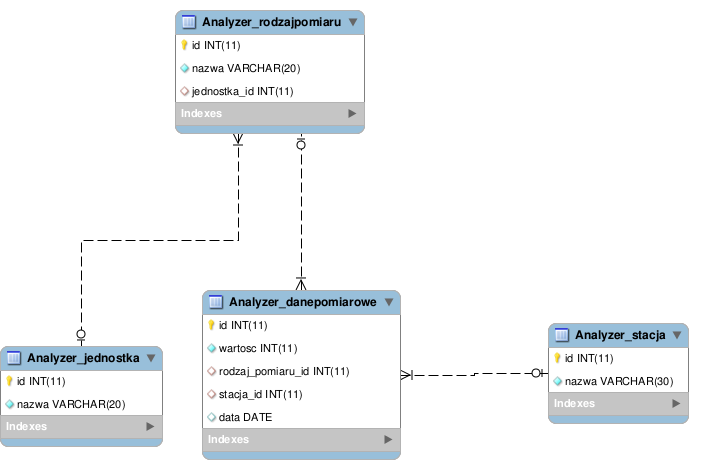
\includegraphics[width=0.8\textwidth]{./diagramEER}
  \caption{Podgląd tabel oraz powiązania pomiędzy nimi w aplikacji.}
  \label{fig:diagram_eer}
\end{figure}

\begin{figure}[htbp]
  \centering
  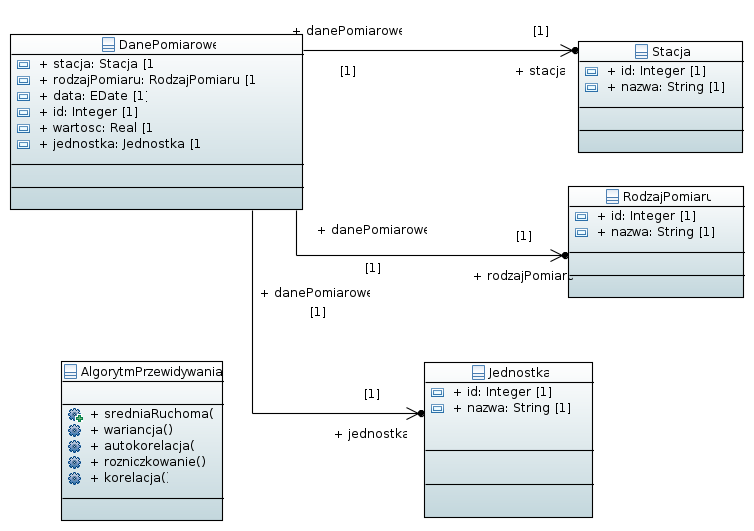
\includegraphics[width=0.8\textwidth]{./uml}
  \caption{Graficzne przedstawienie klas używanych w aplikacji.}
  \label{fig:diagram_uml}
\end{figure}

\section{Algorytm}

Algorytm prognozy bedzie wykorzystywał różne funkcje: średnią ruchomą, wariancję, korelacje i autokorelacje, różniczkowanie.


\section{Interfejs użytkownika}
\end{document}
